\section{Техническое задание}
\subsection{Основание для разработки}

Основанием для разработки является задание на выпускную квалификационную работу бакалавра "<Разработка web сервиса фриланс-биржи">.

\subsection{Цель и назначение разработки}

Основной задачей выпускной квалификационной работы является разработка web-сервиса, реализующего возможности фриланс биржи.

Посредством разработки web-сервиса планируется реализовать возможности фриланс-биржи. Исходя из этого, основную цель предлагается рассмотреть в разрезе двух групп подцелей.

Задачами данной разработки являются:
\begin{itemize}
\item создание сущностей исполнителя и заказчика;
\item реализация функций взаимодействия между данными сущностями;
\item реализация формы просмотра задачи;
\item реализация системы удержания средств до выполнения задания;
\item реализация графического отображения функций сайта для взаимодействия с пользователем.
\end{itemize}

\subsection{Описание проекта "<FreelanceDay!">}

Данный сервис представляет собой систему взаимодействия между двумя типами пользователей -- заказчик и исполнитель. Взаимодействие обоих типов пользователей происходит вокруг задач. Так же, на равне с задачами, пользователи имеют дело с платёжной системой, которая является прикреплённым вознаграждением за задачи. Взаимодействие пользователя с самим сервисом происходит на основе клиент-серверной архитектуры.

Сервис можно разделить на 3 взаимодействующие между собой подсистемы: администрирование (administration), система задач (task system) и платёжная система (payment system).

\subsubsection{Подсистема "<Администрирование">. Сущности исполнителя и заказчика}

Подсистема "<Администрование"> отвечает за хранение информации о пользователях, определение их роли а так же за авторизацию на сайте. Всего в сервисе существует 2 типа пользователя -- заказчик и исполнитель. У каждой из сущностей есть свой набор полей, который частично отличается. 

Сущность заказчика -- это "поставщик" задач. Он может выкладывать на сервис задачи, выбирать кандидатов из списка откликнувшихся и завершать задачу. После полного выполнения заказчик может оставить оценку на исполнителя.

Сущность исполнителя -- это "охотник" на задачи. Он выбирает из списка готовых на сервисе задач, оставляет отклик и берётся за выполнение задачи. После выполнения задачи исполнитель получает очки опыта, которые позволяют повысить уровень, который помогает получать более сложные и высокооплачиваемые задачи.

\subsubsection{Подсистема "<Система задач">. Сущность задачи}

Подсистема "<Система задач"> представляет собой воплощение сущности "<Задача">. Напрямую с данной подсистемой взаимодействуют сущности заказчика и исполнителя.

Сущность задачи -- это объект, который создаётся заказчиком на сервисе с помощью специальных инструментов, представленных сайтом. Заказчик описывает данный объект такими основными признаками, как название задачи, её описание, стоимость и сложность выполнения задачи. После создания она находится в списке доступных для отклика задач и спустя время она обрастает таковыми. Когда исполнитель выбран -- объект находится в статусе, который условно можно назвать "<На выполнении">. Если исполнитель выполнил задачу - он переводит задачу в статус "<На завершении">, а заказчик в свою очередь переводит задачу в статус "<Завершено">, после чего происходит взаимодействие с подсистемой "<Платёжная система"> для перевода средств на виртуальный счёт исполнителя.

\subsubsection{Подсистема "<Платёжная система">. Сущности виртуального счёта и платежа}

Подсистема "<Платёжная система"> представляет собой воплощение сущностей "<Виртуальный счёт"> и "<Платёж"> и предназначена для управления денежными средствами, которые находятся внутри сервиса. 

Сущность виртуального счёта -- это объект, который является вместилещем для денежных средств кадого пользователя и задачи. В зависимости от роли у счёта могут меняться права, например: для роли заказчика счёт доступен только на внесение средств и исходящий перевод, для роли исполнителя наоборот -- только на вывод и входящий перевод, а для счёта сущности задачи доступен на входящие и исходящие переводы.

Сущность платежа -- это объект, который можно назвать "<перевозчиком"> платежей. Т. е. он забирает денежные средства из одной точки (первый виртуальный счёт) и привозит их во вторую точку (второй виртуальный счёт). Так же данный объект используется, как хранитель истории операций -- можно просмотреть когда проходил платёж, отравителя, получателя и его сумму.

\subsection{Требования пользователя к web сервису}

Сервис должен включать в себя следующий функционал:
\begin{itemize}
    \item авторизация пользователя;
    \item регистрация на сервисе;
    \item отображение личного кабинета пользователя;
    \item пополнение средств заказчиком;
    \item вывод средств пользователем;
    \item отображение списка доступных задач;
    \item создание задачи заказчиком, зачисление на неё средств;
    \item отображение информации о задаче;
    \item отклик на задачу исполнителями;
    \item выбор исполнителя заказчиком из списка кандидатов;
    \item завершение выполнения задачи со стороны как исполнителя, так и заказчика;
    \item перечисление средств за выполнение задачи на виртуальный счёт исполнителя.
\end{itemize}

На рисунке ~\ref{tz1:image} представлен макет страницы просмотра доступных задач.

\begin{figure}[ht]
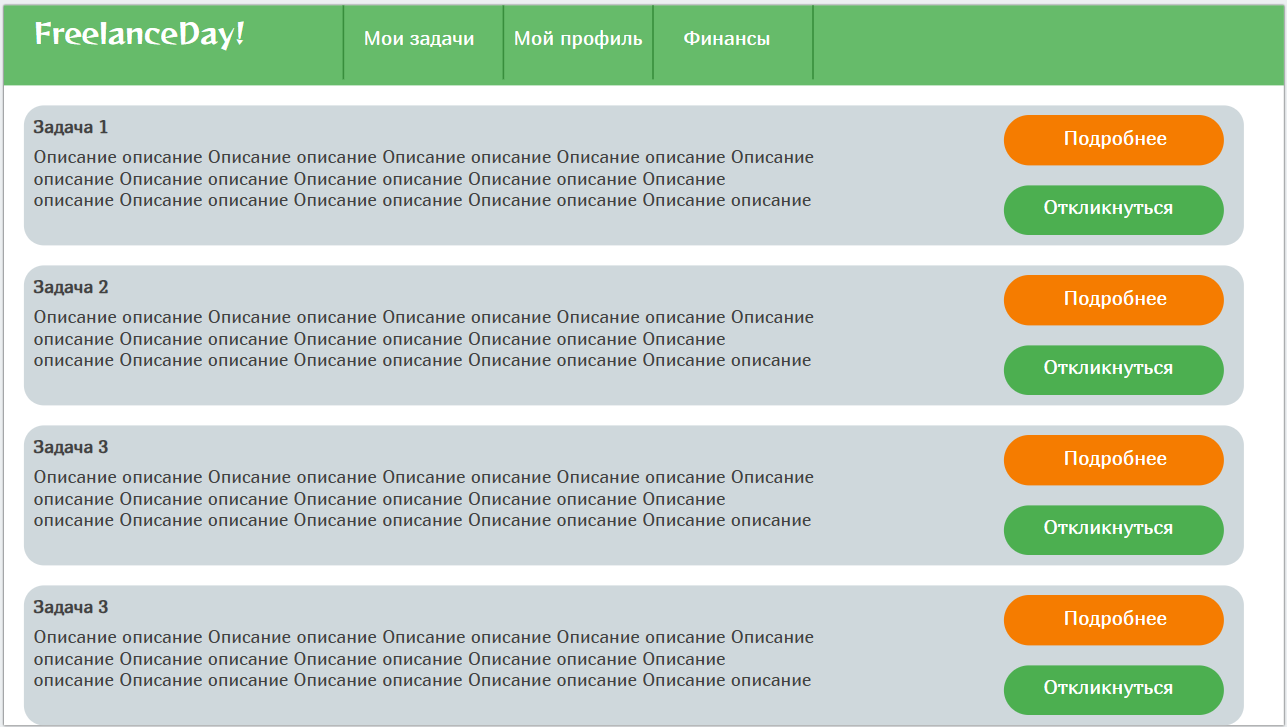
\includegraphics[width=1\linewidth]{tz0s1.png}
\caption{Макет страницы просмотра доступных задач}
\label{tz1:image}
\end{figure}
%\vspace{-\figureaboveskip} % двойной отступ не нужен (можно использовать, если раздел заканчивается картинкой)

Здесь представлены сами задачи, их краткое описание и кнопки для отклика на задачу и для просмотра подробной информации о задаче. Так же на каждой странице можно увидеть кнопки в шапке страницы -- "<Мои задачи">, "<Мой профиль"> и "<Финансы"> -- они переносят пользователя на соответствующую страницу.

На рисунке ~\ref{tz2:image} представлен макет страницы входа на сайт.
\clearpage

\begin{figure}[ht]
	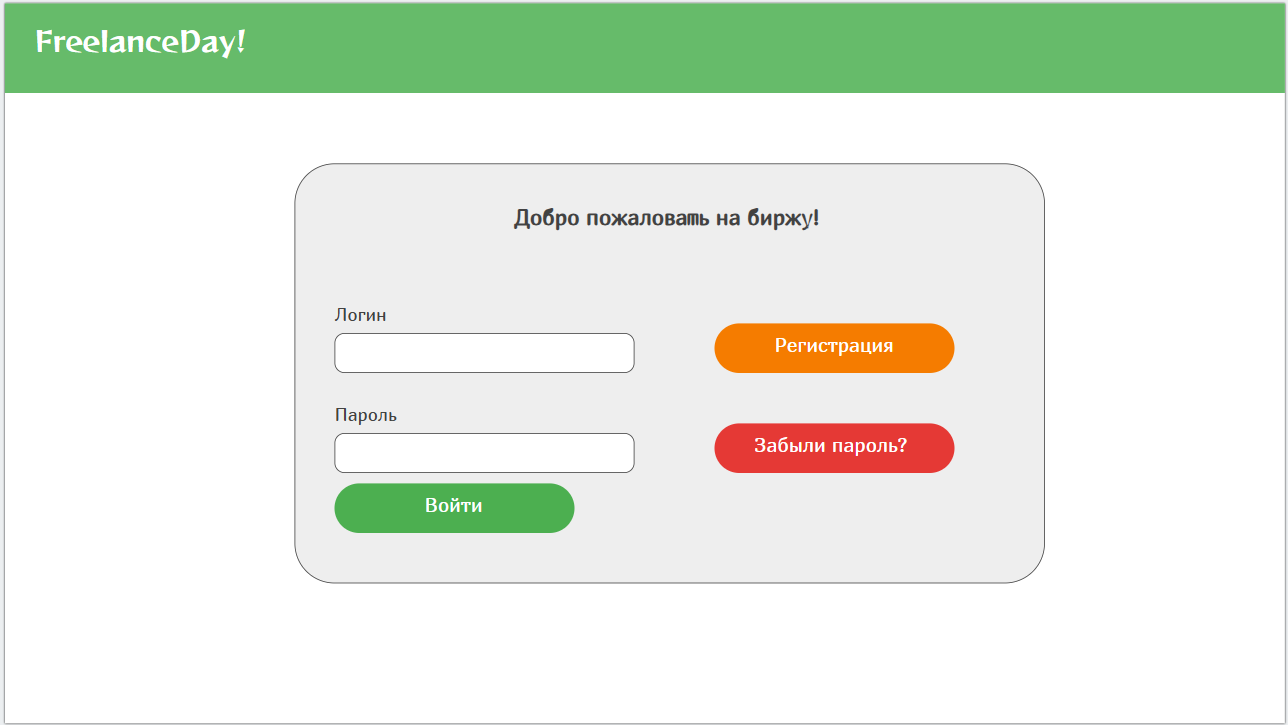
\includegraphics[width=1\linewidth]{tz0s2.png}
	\caption{Макет страницы входа на сайт}
	\label{tz2:image}
\end{figure}

Здесь представлены поля для вввода логина, пароля, кнопки для входа на сайт, перехода на страницу регистрации и для перехода на страницу восстановления пароля.

На рисунке ~\ref{tz3:image} представлен макет страницы просмотра информации о пользователе.
\clearpage

\begin{figure}[ht]
	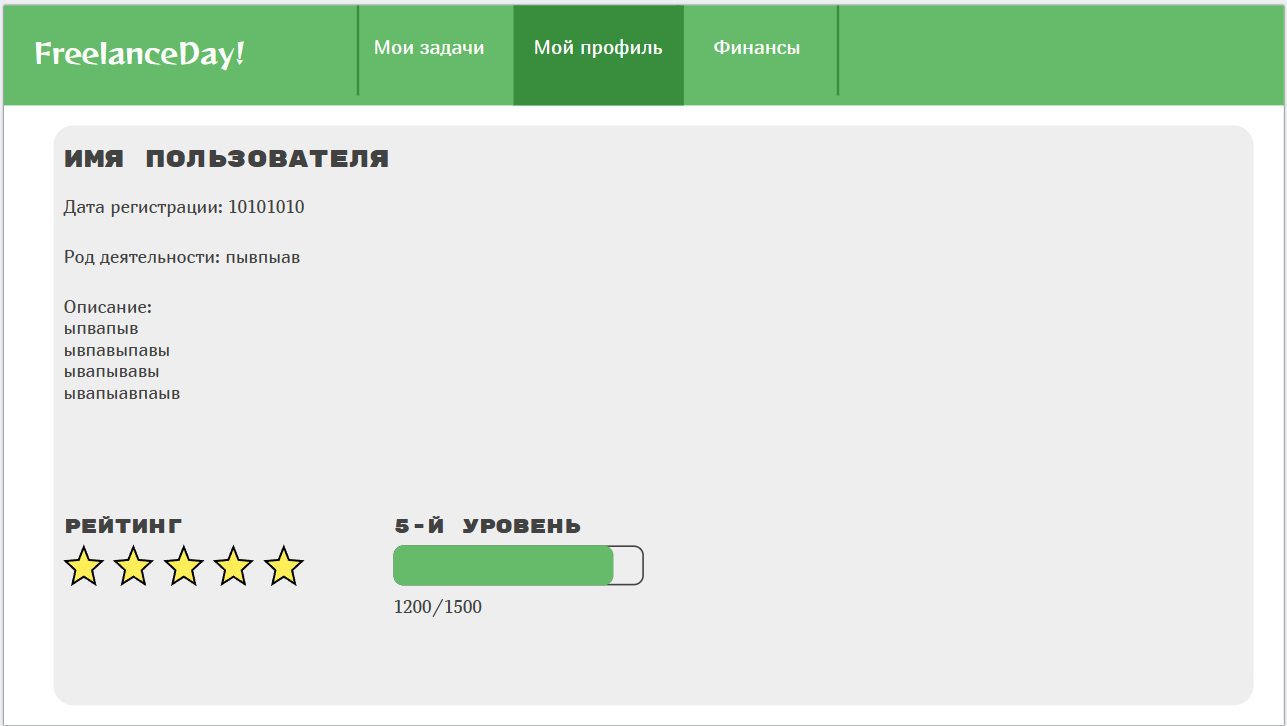
\includegraphics[width=1\linewidth]{tz0s3.png}
	\caption{Макет страницы просмотра информации о пользователе}
	\label{tz3:image}
\end{figure}

Здесь представлены поля, которые отображают доступную информацию о пользователе - его имя, дату регистрации, описание пользователя, рейтинг на сервисе и уровень.

\subsection{Моделирование вариантов использования}

\subsubsection{Диаграмма прецедентов}

Для разрабатываемого сайта была реализована модель, которая обеспечивает наглядное представление вариантов использования сайта.

Она помогает в физической разработке и детальном анализе взаимосвязей объектов. При построении диаграммы вариантов использования применяется унифицированный язык визуального моделирования UML.

Диаграмма вариантов описывает функциональное назначение разрабатываемой системы. То есть это то, что система будет непосредственно делать в процессе своего функционирования. Она является исходным концептуальным представлением системы в процессе ее проектирования и разработки. Проектируемая система представляется в виде ряда прецедентов, предоставляемых системой актерам или сущностям, которые взаимодействуют с системой. Актером или действующим лицом является сущность, взаимодействующая с системой извне (например, человек, техническое устройство). Прецедент служит для описания набора действий, которые система предоставляет актеру.

На основании анализа предметной области в программе должны быть реализованы следующие прецеденты:
\begin{itemize}
\item авторизация пользователя, определение роли;
\item пополнение виртуального счёта заказчика;
\item создание задачи и перечисление на неё средств;
\item выбор исполнителя;
\item завершение задачи;
\item просмотр списка доступных задач;
\item просмотр подробной информации о задаче;
\item отклик на задачу;
\item отправка задачи на завершение;
\item вывод средств с виртуального счёта исполнителя;
\item выход из аккаунта.
\end{itemize}
\clearpage

\begin{figure}[ht]
	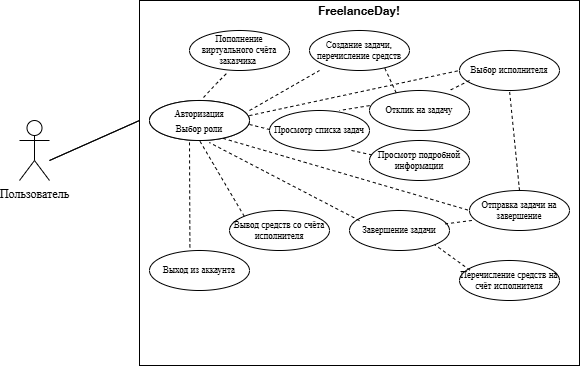
\includegraphics[width=1\linewidth]{useCase.png}
	\caption{Диаграмма прецедентов}
	\label{ucUML:image}
\end{figure}

\subsubsection{Сценарии прецедентов программы}


\paragraph{Сценарий для прецедента "<Авторизация пользователя, определение роли">}

Основной исполнитель: пользователь.

Заинтересованные лица и их требования: пользователю необходимо произвести вход на сайт.

Предусловие: перед началом работы у пользователя открыта страница входа на сайт.

Основной успешный сценарий:

\begin{enumerate}
	\item Пользователь заполняет поля "<Логин"> и "<Пароль"> валидными значениями. 
	\item Пользователь нажимает кнопку "<Войти">. 
	\item Отображается главная страница сайта, материал на странице представлен в зависимости от роли пользователя.
\end{enumerate} 

\paragraph{Сценарий для прецедента "<Пополнение виртуального счёта заказчика">}

Основной исполнитель: пользователь с ролью "<Заказчик">.

Заинтересованные лица и их требования: пользователю необходимо пополнить свой виртуальный счёт.

Предусловие: пользователь авторизован на сайте, открыта страница пополнения виртуального счёта.

Основной успешный сценарий: 

\begin{enumerate}
	\item Пользователь заполняет необходимые поля данными своей карты и поле "<Сумма пополнения"> необходимой суммой, которую хочет получить на свой виртуальный счёт. 
	\item Пользователь нажимает кнопку "<Пополнить">, подтверждает свою карту. \item Отображается информационное сообщение об успешном пополнении, сумма виртуального счёта увеличена на сумму пополнения.
\end{enumerate}
		
\paragraph{Сценарий для прецедента "<Создание задачи и перечисление на неё средств">}

Основной исполнитель: пользователь с ролью "<Заказчик">.

Заинтересованные лица и их требования: пользователю необходимо создать задачу.

Предусловие: пользователь авторизован на сайте, у пользователя пополнен виртуальный счёт, открыта страница создания задачи.

Основной успешный сценарий: 

\begin{enumerate}
	\item Пользователь заполняет обязательные поля информацией о задаче, поле "<Сумма"> заполняет валидным значением средств.
	\item Пользователь нажимает кнопку "<Создать задачу">. 
	\item Отображается информационное сообщение "<Задача успешно создана">.
\end{enumerate}

\paragraph{Сценарий для прецедента "<Выбор исполнителя">}

Основной исполнитель: пользователь с ролью "<Заказчик">.

Заинтересованные лица и их требования: пользователю необходимо выбрать исполнителя на задачу.

Предусловие: пользователь авторизован на сайте, задача в статусе "<Создана"> пользователем создана задача, на задачу откликнулось несколько исполнителей, открыта страница просмотра кандидатов по задаче.

Основной успешный сценарий: 

\begin{enumerate}
	\item Пользователь просматривает информацию о кандидатах. 
	\item Пользователь выбирает исполнителя путём нажатия кнопки "<Выбрать"> в поле соответствующего исполнителя. 
	\item Отображается информационное сообщение "<Исполнитель успешно выбран"> и информация об выбранном исполнителе.
\end{enumerate}

\paragraph{Сценарий для прецедента "<Завершение задачи">}

Основной исполнитель: пользователь с ролью "<Заказчик">.

Заинтересованные лица и их требования: пользователю необходимо завершить задачу.

Предусловие: пользователь авторизован на сайте, открыта страница с информацией о задаче, на задачу назначен исполнитель и она в статусе "<На завершении">.

Основной успешный сценарий: 

\begin{enumerate}
	\item Пользователь нажимает кнопку "<Завершить">. 
	\item Отображается информационное сообщение "<Задача успешно завершена">, задача в статусе "<Завершена">, средства с виртуального счёта задачи перечисляются на виртуальный счёт закреплённого исполнителя.
\end{enumerate}

\paragraph{Сценарий для прецедента "<Просмотр списка доступных задач">}

Основной исполнитель: пользователь с ролью "<Исполнитель">.

Заинтересованные лица и их требования: пользователю необходимо просмотреть список доступных задач.

Предусловие: пользователь авторизован на сайте, открыта страница просмотра списка задач.

Основной успешный сценарий: отображается список доступных задач. У каждой задачи отображаются поля с информацией о задаче и кнопки: "<Подробнее"> и "<Откликнуться">.

\paragraph{Сценарий для прецедента "<Просмотр подробной информации о задаче">}

Основной исполнитель: пользователь с ролью "<Исполнитель">.

Заинтересованные лица и их требования: пользователю необходимо посмотреть подробную информацию о задаче.

Предусловие: пользователь авторизован на сайте, открыта страница просмотра списка задач.

Основной успешный сценарий:

\begin{enumerate}
	\item Пользователь нажимает кнопку "<Подробнее"> на необходимой задаче. 
	\item Отображается страница просмотра полной информации о задаче.
\end{enumerate}

\paragraph{Сценарий для прецедента "<Отклик на задачу">}

Основной исполнитель: пользователь с ролью "<Исполнитель">.

Заинтересованные лица и их требования: пользователю необходимо откликнуться на выбранную задачу.

Предусловие: пользователь авторизован на сайте, открыта страница просмотра задач.

Основной успешный сценарий: 

\begin{enumerate}
	\item Пользователь нажимает кнопку "<Откликнуться"> на выбранной задаче. 
	\item Кнопка "<Откликнуться"> не отображается, отображается информационное сообщение "<Отклик успешно отправлен!">.
\end{enumerate}

\paragraph{Сценарий для прецедента "<Отправка задачи на завершение">}

Основной исполнитель: пользователь с ролью "<Исполнитель">.

Заинтересованные лица и их требования: пользователю необходимо задачу, которая находится у него в работе, отправить на завершение.

Предусловие: пользователь авторизован на сайте и назначен на задачу, которая находится в статусе "<В работе">, открыта страница просмотра информации о задаче.

Основной успешный сценарий: 
	
\begin{enumerate}
	\item Пользователь нажимает кнопку "<Отправить на завершение">. 
	\item Кнопка "<Отправить на завершение"> не отображается, отображается информационное сообщение "<Задача успешно отправлена на завершение!">, задача в статусе "<На завершении">.
\end{enumerate}	

\paragraph{Сценарий для прецедента "<Вывод средств с виртуального счёта исполнителя">}

Основной исполнитель: пользователь с ролью "<Исполнитель">.

Заинтересованные лица и их требования: пользователю необходимо вывести средства со своего виртуального счёта на банковскую карту.

Предусловие: пользователь авторизован на сайте и на его виртуальном счёте присутствуют денежные средства, открыта страница вывода средств.

Основной успешный сценарий: 
	
\begin{enumerate}
	\item Пользователь заполняет необходимые поля информацией о банковской карте, поле "<Сумма вывода"> валидным значением, нажимает кнопку "<Вывести">, подтверждает банковскую карту. 
	\item Отображается информационное сообщение "<Средства успешно отправлены!">, сумма виртуального счёта пользователя уменьшилась на сумму вывода.
\end{enumerate}

\paragraph{Сценарий для прецедента "<Выход из аккаунта">}

Основной исполнитель: пользователь.

Заинтересованные лица и их требования: пользователю необходимо произвести выход из аккаунта.

Предусловие: пользователь авторизован, открыта страница информации о пользователе.

Основной успешный сценарий:
	
\begin{enumerate}
	\item Пользователь нажимает кнопку "<Выйти из аккаунта">. 
	\item Отображается страница входа на сайт.
\end{enumerate}

\subsection{Требования к оформлению документации}

Разработка программной документации и программного изделия должна производиться согласно ГОСТ 19.102-77 и ГОСТ 34.601-90. Единая система программной документации.
